\chapter{Dataset, Experimental Methodology and Evaluation}
\label{ch:dataset_and_evaluation}

This chapter describes the data the expert system was tested on (Sections~\ref{sec:dataset} and~\ref{sec:testcases}), how the experiments were designed and validated (Sections~\ref{sec:design} and~\ref{sec:validation}), how performance was measured (Section~\ref{sec:metrics}) and what the results show (Sections~\ref{sec:results} and~\ref{sec:sensitivity}). Every table of results in this chapter is generated by the test code from the current knowledge base and datasets, so the numbers can be reproduced exactly (Chapter~\ref{ch:software_and_reproducibility}).

% ---------------------------------------------------------------------------
\section{Dataset and Data Dictionary}
\label{sec:dataset}

\subsection{Data origin}

\textbf{Every test case in this project is synthetic.} No measured fault data from a real data centre were available, and no value in the dataset is presented as a real measurement. The project framework requires four kinds of information to be kept apart, and they are kept apart as follows:

\begin{itemize}
  \item \textbf{Measured data:} none.
  \item \textbf{Synthetic test cases:} generated by a physics simulator, or written by hand for four smoke tests. Every case carries the origin \texttt{synthetic} in its \texttt{case/3} fact.
  \item \textbf{Engineering assumptions:} recorded as sources of type \texttt{assumption} in the knowledge base (Table~\ref{tab:provenance}), and listed for the simulator in Table~\ref{tab:sim-assumptions}.
  \item \textbf{Literature-supported rules:} rules whose source is of type \texttt{standard} or \texttt{literature}.
\end{itemize}

\subsection{The simulator}

The test cases were generated by a steady-state simulator of the row, written in Python with only the standard library. It implements the engineering model of Section~\ref{sec:maths}. Each case is built in four steps:

\begin{enumerate}
  \item \textbf{Workload.} The row load is drawn as low, nominal or high, at mean utilisations of 10 to 20\%, 40 to 60\% or 80 to 90\%. Each rack varies around the row value and each server around its rack.
  \item \textbf{Fault injection into the physics.} A fault changes a physical parameter, never a reading directly. A fan failure, for example, reduces the airflow the fan delivers, and every temperature then follows from the physics. Table~\ref{tab:fault-params} lists the parameter changed for each fault.
  \item \textbf{Steady-state solution.} The coupled server, rack, cooling-unit and coil equations are solved by damped fixed-point iteration. The cooling-unit fan follows the airflow demand of the servers, and the valve controller finds the smallest opening that holds the 20\,\textdegree C setpoint.
  \item \textbf{Sensor layer.} Sensor bias, Gaussian measurement noise, frozen readings for stale telemetry and randomly missing readings are applied last.
\end{enumerate}

Because faults act on the physics, their symptoms arise as consequences rather than being written in. The diagnostic rules are therefore tested against behaviour they were not built from, which is what exposed the three knowledge-base errors described in Section~\ref{sec:acquisition}.

\begin{table}[htbp]
  \centering
  \small
  \caption{Physical parameter changed for each injected fault.}
  \label{tab:fault-params}
  \begin{tabular}{L{3.2cm}L{6.4cm}L{2.2cm}L{2.2cm}}
    \toprule
    Fault & Parameter changed & Clear range & Borderline range \\
    \midrule
    $F_1$ CRAH fan failure & Airflow fraction delivered; fan power over prediction & 0 to 0.1; 0.05 to 0.15 & 0.3 to 0.5; 0.4 to 0.6 \\
    $F_2$ chilled-water loss & Fraction of design water flow available & 0.02 to 0.2 & 0.25 to 0.4 \\
    $F_3$ filter clogging & Filter loading ratio, Equation E27 & 3 to 6 & 1.8 to 2.5 \\
    $F_4$ recirculation & Extra recirculation fraction at the top of one rack & 0.25 to 0.5 & 0.12 to 0.2 \\
    $F_5$ server fan failure & Server airflow and reported fan speed near zero & -- & -- \\
    $F_6$ branch overload & Phase 1 share of feed A, set for a target current & 27 to 30\,A & 24.5 to 26.5\,A \\
    $F_7$ battery degradation & Cell resistance ratio, with low float voltage & 1.5 to 2.5 & 1.2 to 1.4 \\
    $F_8$ UPS on bypass & Mode flag; efficiency rises to 0.99 & -- & -- \\
    $S_1$ sensor bias & Offset on one inlet or supply-air sensor & 3 to 8\,K & -- \\
    $S_2$ telemetry dropout & One telemetry group frozen, sample age 300 to 1800\,s & -- & -- \\
    \bottomrule
  \end{tabular}
\end{table}

\begin{table}[htbp]
  \centering
  \small
  \caption{Main simulator assumptions.}
  \label{tab:sim-assumptions}
  \begin{tabular}{L{3.8cm}L{5.4cm}L{4.8cm}}
    \toprule
    Assumption & Value & Reason \\
    \midrule
    Server power & 0.40\,kW idle, 0.90\,kW at full load, 55\% in the CPU & Equation E1; a typical two-socket server (to verify) \\
    Server airflow & 0.055\,kg/s at nominal fan speed & Gives a 13 to 16\,K rise across a server \\
    CPU throttling & Clock reduced to keep the CPU at or below 95\,\textdegree C & Vendor limits vary (to verify) \\
    Cooling-unit fan control & Supplies 10\% more air than the servers demand & Common practice to limit recirculation \\
    Coil heat transfer & 15\,kW/K air side; 10\,kW/K water side at 3.2\,kg/s, scaling with flow to the power 0.8 & Gives a 5 to 7\,K water temperature rise in normal operation \\
    Airflow shortfall & 40\% drawn from the hot aisle, 60\% from room air at 25\,\textdegree C & Without it a fan failure has no steady state \\
    Power distribution & Two feeds per rack sharing the load equally & Standard 2N practice \\
    Measurement noise & 0.15\,K on air temperatures; 1\% on power and current & Typical sensor accuracy (to verify) \\
    Time & Steady state only & A limitation: transients are not modelled \\
    \bottomrule
  \end{tabular}
\end{table}

\subsection{Data dictionary}

The variables, units and sensors are defined in Table~\ref{tab:variables}. Each case has about 460 readings: nine for the cooling unit, six for each rack, one current for each of the six phase circuits of each rack, three for each of the 120 servers, six for the UPS and battery, and one sample age for each telemetry group. The simulator writes every dataset in three forms: Prolog facts for the expert system, a CSV file in long format with units for analysis outside Prolog, and a JSON file holding the hidden ground truth of each case, such as the injected severities.

\subsection{Datasets}

Four datasets were used (Table~\ref{tab:datasets}). The calibration and held-out splits have the same composition but different random seeds. A fixed seed always reproduces the same cases.

\begin{table}[htbp]
  \centering
  \small
  \caption{Datasets.}
  \label{tab:datasets}
  \begin{tabular}{L{3.0cm}L{2.0cm}L{2.2cm}L{6.8cm}}
    \toprule
    Dataset & Cases & Seed & Use \\
    \midrule
    Smoke tests & 4 & -- & Hand-written cases for the explanation demonstrations \\
    Calibration & 255 & 20261020 & Checking thresholds and signatures during development \\
    Held-out & 255 & 777 & Reported performance; never used to adjust anything \\
    Sensitivity sweeps & 24 $\times$ 60 & 4242 to 4545 & Sensitivity to noise, missing data, multiple faults and sensor bias \\
    \bottomrule
  \end{tabular}
\end{table}

% ---------------------------------------------------------------------------
\section{Test Cases}
\label{sec:testcases}

The calibration and held-out splits each contain seven categories, which together cover the eight test categories that the project framework requires (Table~\ref{tab:test-categories}). Test~H, explanation and maintenance, is assessed on every case through ExplainabilityRate and PlanValidity, and demonstrated in full by the explanation traces of Section~\ref{sec:explanation}.

\begin{table}[htbp]
  \centering
  \small
  \caption{Test categories and the framework tests they cover.}
  \label{tab:test-categories}
  \begin{tabular}{L{2.6cm}L{1.0cm}L{1.6cm}L{8.8cm}}
    \toprule
    Category & Cases & Test & Contents \\
    \midrule
    Normal & 30 & A & 10 cases each at low, nominal and high load \\
    Single fault & 120 & B, C, D & 15 cases of each physical fault $F_1$ to $F_8$ \\
    Instrumentation & 30 & E & 15 sensor-bias and 15 telemetry-dropout cases \\
    Multiple & 30 & F & 6 cases of each combination in Table~\ref{tab:interactions} \\
    Incomplete & 15 & G & A random single fault or normal case with 15\% of readings removed \\
    High noise & 15 & G & A random single fault with five times the nominal sensor noise \\
    Borderline & 15 & G & Fault severities near or below the detection thresholds, and high-load normal cases \\
    All categories & 255 & H & Explanation and maintenance plan for every diagnosis \\
    \bottomrule
  \end{tabular}
\end{table}

The borderline category deliberately includes faults injected below the detection thresholds. Its exact-match score is therefore expected to be low, and it is reported to measure how gracefully detection degrades, not as a target to maximise.

% ---------------------------------------------------------------------------
\section{Experimental Design}
\label{sec:design}

Figure~\ref{fig:evaluation} shows the experimental workflow. Three design decisions protect the results against optimistic bias.

\begin{figure}[htbp]
  \centering
  % Figure 8: experimental and evaluation workflow.
\begin{tikzpicture}[x=1cm, y=1cm]
  \node[data=4.4cm, align=left] (sim) at (0.6,0)
    {\textbf{Physics simulator}\\
     \footnotesize steady-state model, Stage 4\\
     \footnotesize faults injected into the physics\\
     \footnotesize sensor layer: noise, bias,\\
     \footnotesize \quad stale and missing data};
  \node[data=3cm] (hand) at (0.6,-2.6) {Hand-written smoke cases};

  \node[data=3.4cm] (cal) at (5.9,1.3) {Calibration split\\ \footnotesize 255 cases, seed 20261020};
  \node[data=3.4cm] (hold) at (5.9,-0.1) {Held-out split\\ \footnotesize 255 cases, seed 777};
  \node[data=3.4cm] (swp) at (5.9,-1.5) {Sensitivity sweeps\\ \footnotesize 24 sets of 60 cases};

  \node[reason=3.2cm] (pl) at (10.6,-0.1) {Prolog, four reasoning modes};
  \node[out=3.2cm] (met) at (10.6,-2.0) {Metrics\\ \footnotesize \texttt{tests/metrics.pl}};
  \node[out=3.7cm] (sen) at (10.6,-3.4) {Sensitivity analysis\\ \footnotesize \texttt{tests/sensitivity.py}};
  \node[kb=3.4cm] (kb) at (5.9,3.2) {Knowledge base};

  \draw[flow] (sim.east) -- ++(0.4,0) |- (cal.west);
  \draw[flow] (sim.east) -- ++(0.4,0) |- (hold.west);
  \draw[flow] (sim.east) -- ++(0.4,0) |- (swp.west);
  \draw[flow] (hand.east) -- (8.45,-2.6) |- (pl.west);
  \draw[flow] (cal.east) -- ++(0.5,0) |- (pl.west);
  \draw[flow] (hold) -- (pl);
  \draw[flow] (swp.east) -- ++(0.5,0) |- (pl.west);
  \draw[flow] (pl) -- (met);
  \draw[flow] (met) -- (sen);
  \draw[uses] (kb.east) -| (pl.north);
  \draw[feedback] (cal.north) -- node[tag, right] {threshold checks, rule fixes} (kb.south);
  \node[note] at (4.6,-3.55) {the held-out split is never used to tune anything};
\end{tikzpicture}

  \caption{Experimental and evaluation workflow, with the calibration and held-out splits kept apart.}
  \label{fig:evaluation}
\end{figure}

\paragraph{Calibration and held-out splits.} Thresholds were set from engineering reasoning and then checked against the calibration split, by profiling each signature in normal and fault cases. The held-out split was generated afterwards with a different seed and was never used to choose or adjust anything. Its results are the reported performance.

\paragraph{Faults in the physics, not the readings.} Because the simulator injects faults into the physical model, the knowledge base cannot simply reproduce the generator's rules. Symptoms that the knowledge base did not anticipate appear in the data, as the three errors found during development show.

\paragraph{Four configurations on identical data.} The four reasoning configurations of Section~\ref{sec:inference} run on exactly the same cases, so differences between them are due to the reasoning alone. This comparison is the ablation study that the framework asks for.

Reasoning time is measured as wall-clock time per case, after a warm-up pass and with the symptom cache cleared for each case, so that every configuration pays the full cost of its own evidence computation.

% ---------------------------------------------------------------------------
\section{Validation}
\label{sec:validation}

Verification asks whether the system implements its design correctly. Validation asks whether the design is right for the problem. Both were addressed at several levels:

\begin{itemize}
  \item \textbf{Equations against physics.} The simulator's normal cases were checked against independent hand calculations. A 78\,kW row needs about 4.9\,m$^3$/s of air at a 13\,K rise, and the fan figures imply a plausible pressure rise of about 225\,Pa. The coil model was tuned so that normal operation gives the 5 to 7\,K water temperature rise of real chilled-water coils.
  \item \textbf{Rules against simulated physics.} Each new rule was first run against the calibration split. Rules that disagreed with the physics were revised rather than the data, which exposed the three errors of Section~\ref{sec:acquisition}.
  \item \textbf{Generalisation.} The held-out split measures performance on cases that played no part in development. Held-out accuracy is slightly higher than calibration accuracy for every configuration (Tables~\ref{tab:modes-holdout} and~\ref{tab:modes-calibration}), which makes overfitting to the calibration split unlikely. Both splits come from the same simulator, however, so this tests generalisation across cases of one model, not to a different system. Section~\ref{sec:mismatch} tests robustness to the model itself.
  \item \textbf{Explanations.} Explanation traces were inspected for representative cases of every category. The trace of Listing~\ref{lst:why} shows each element that the framework requires.
  \item \textbf{Regression.} The four smoke cases and both splits are rerun after every change to the knowledge base.
\end{itemize}

The main limitation of this validation is that both the knowledge base and the simulator rest on the same engineering model. Agreement between them shows that the reasoning is consistent with the model, not that the model is consistent with a real data centre. Section~\ref{sec:mismatch} measures how much the results depend on the model being exactly right, by regenerating the held-out cases with deliberately changed physics. Validation on measured data remains future work (Chapter~\ref{ch:conclusion}).

% ---------------------------------------------------------------------------
\section{Metrics}
\label{sec:metrics}

The metrics follow Section~\ref{sec:maths}. Because a case can contain several faults, each metric is counted as follows:

\begin{itemize}
  \item \textbf{Exact match} is the share of cases whose predicted set of fault labels equals the true set exactly. A label names both the fault and the affected entity, so diagnosing recirculation at the wrong rack counts as wrong.
  \item \textbf{Coverage} is the share of cases in which every true fault was predicted, whether or not extra faults were predicted too.
  \item \textbf{Precision, recall and F1-score} are computed for each fault class from label-level counts: a predicted label that matches a true label is a true positive. Macro averages are taken over the eleven classes.
  \item \textbf{Class accuracy} is the framework's Equation~\eqref{eq:metrics} at case level: for each class, the share of cases in which the presence or absence of that class was predicted correctly. Its mean over the classes is reported.
  \item \textbf{ExplainabilityRate} is the share of cases in which every reported label has a justification, meaning a deductive proof, a clearly present supporting symptom or a hit conflict set, together with a maintenance plan and sourced thresholds. The system only reports a label for one of these reasons, so this rate cannot fall below 100\%. It confirms that every output is traceable, not that the explanation is the real reason for the output. Explanation fidelity, below, tests that.
  \item \textbf{Explanation fidelity} removes the observations an explanation cites and diagnoses the case again (Section~\ref{sec:fidelity}). Unlike ExplainabilityRate, it can fail.
  \item \textbf{PlanValidity} is the share of issued maintenance plans that address a fault really present. A routine plan counts as valid only for a truly normal case. One plan is issued per label, and a plan counts as valid when its label is correct, so PlanValidity is in effect label-level precision. It does not test whether a plan's actions are the right ones. That rests on the plans' sources and verification steps (Section~\ref{sec:planner}), and ideally on review by a practitioner.
  \item \textbf{Reasoning time} is the mean and maximum wall-clock time per case.
\end{itemize}

Confidence scores are used only to rank hypotheses. No probability is claimed, so probabilistic metrics such as calibration curves are not reported.

% ---------------------------------------------------------------------------
\section{Results}
\label{sec:results}

\subsection{Overall performance}

Table~\ref{tab:modes-holdout} gives the held-out results of the four configurations, and Table~\ref{tab:modes-calibration} the calibration results for comparison. Each exact-match rate is given with its Wilson 95\% confidence interval. Because all four configurations diagnose the same cases, they are compared pairwise with an exact McNemar test on the cases where they disagree (Table~\ref{tab:significance-holdout}).

% Generated by tests/metrics_latex.pl. Do not edit by hand.
\begin{table}[htbp]
  \centering
  \footnotesize
  \setlength{\tabcolsep}{4pt}
  \caption{Comparison of reasoning modes, held-out split (255 cases). Class acc.: mean class accuracy. Explain.: ExplainabilityRate. Plan val.: PlanValidity.}
  \label{tab:modes-holdout}
  \begin{tabular}{L{3.4cm}rrrrrrr}
  \toprule
  Mode & Exact & Coverage & Macro F1 & Class acc. & Mean ms & Explain. & Plan val. \\
  \midrule
  Deductive only & 91.0\% & 95.7\% & 0.924 & 98.6\% & 0.22 & 100.0\% & 85.1\% \\
  Deductive + abductive & 94.5\% & 96.1\% & 0.958 & 99.0\% & 1.09 & 100.0\% & 94.2\% \\
  Deductive + consistency-based & 93.3\% & 97.3\% & 0.950 & 99.0\% & 1.03 & 100.0\% & 91.4\% \\
  Complete system & 93.7\% & 96.5\% & 0.954 & 99.0\% & 1.16 & 100.0\% & 92.9\% \\
  \bottomrule
  \end{tabular}
\end{table}

% Generated by tests/metrics_latex.pl. Do not edit by hand.
\begin{table}[htbp]
  \centering
  \footnotesize
  \setlength{\tabcolsep}{4pt}
  \caption{Comparison of reasoning modes, calibration split (255 cases). 95\% CI: Wilson confidence interval of the exact-match rate. Explain.: ExplainabilityRate. Plan val.: PlanValidity.}
  \label{tab:modes-calibration}
  \begin{tabular}{L{2.9cm}rrrrrrrr}
  \toprule
  Mode & Exact & 95\% CI & Coverage & Macro F1 & Mean ms & Max ms & Explain. & Plan val. \\
  \midrule
  Deductive only & 90.2\% & 85.9--93.3 & 95.3\% & 0.925 & 0.18 & 0.68 & 100.0\% & 86.7\% \\
  Deductive + abductive & 93.3\% & 89.6--95.8 & 94.5\% & 0.954 & 0.95 & 2.52 & 100.0\% & 94.4\% \\
  Deductive + consistency-based & 91.8\% & 87.7--94.6 & 95.3\% & 0.942 & 0.84 & 2.48 & 100.0\% & 91.6\% \\
  Complete system & 93.3\% & 89.6--95.8 & 95.3\% & 0.952 & 0.96 & 3.20 & 100.0\% & 93.8\% \\
  \bottomrule
  \end{tabular}
\end{table}

% Generated by tests/metrics_latex.pl. Do not edit by hand.
\begin{table}[htbp]
  \centering
  \small
  \caption{Paired comparison of reasoning modes, held-out split: exact two-sided McNemar test on the cases where the two modes disagree. Only A: cases the first mode gets right and the second wrong. Holm: $p$ adjusted for the six comparisons by Holm's method. Bold: below 0.05.}
  \label{tab:significance-holdout}
  \begin{tabular}{L{3.6cm}L{3.6cm}rrrr}
  \toprule
  Mode A & Mode B & Only A & Only B & $p$ & Holm \\
  \midrule
  Deductive only & Deductive + abductive & 2 & 11 & \textbf{0.022} & 0.135 \\
  Deductive only & Deductive + consistency-based & 2 & 8 & 0.109 & 0.461 \\
  Deductive only & Complete system & 3 & 10 & 0.092 & 0.461 \\
  Deductive + abductive & Deductive + consistency-based & 5 & 2 & 0.453 & 1.000 \\
  Deductive + abductive & Complete system & 2 & 0 & 0.500 & 1.000 \\
  Deductive + consistency-based & Complete system & 2 & 3 & 1.000 & 1.000 \\
  \bottomrule
  \end{tabular}
\end{table}


Four findings stand out.

\begin{enumerate}
  \item \textbf{Every configuration is accurate on the core categories.} All four diagnose every normal, single-fault and instrumentation case of the held-out split correctly (Table~\ref{tab:categories-holdout}). Over five held-out seeds, they miss 3 to 6 of the 900 such cases (Section~\ref{sec:seeds}).
  \item \textbf{Abduction gives the largest gain.} Adding abduction raises exact-match accuracy from 91.0\% to 94.5\%. It corrects 11 cases that deduction gets wrong and loses 2, a significant difference ($p = 0.022$). The gain comes almost entirely from the imperfect-evidence categories, where parsimony removes spurious findings. On this split, the complete system's gain over deduction is not significant ($p = 0.092$), although it is on the calibration split ($p = 0.039$) and over five seeds.
  \item \textbf{One split cannot separate the model-based configurations; five seeds can.} On the held-out split their exact-match rates differ by two to five cases, their confidence intervals overlap, and no pairwise difference between them approaches significance ($p \ge 0.45$). Pooled over five held-out seeds, every pairwise difference is significant, and deductive + abductive reasoning is the most accurate configuration (Section~\ref{sec:seeds}). Consistency checking is the only mode that catches the smallest supply-sensor bias in the calibration split, and it refuses explanations that leave a violated relation unexplained. Under heavy noise, however, it occasionally takes a chance violation of the power balance at face value and reports a meter fault.
  \item \textbf{Every output is traceable, and the explanations are faithful.} ExplainabilityRate is 100\% in every configuration, as it must be by construction. The fidelity test, which can fail, finds that removing the evidence an explanation cites removes the diagnosis in 96 to 100\% of cases (Section~\ref{sec:fidelity}). Reasoning takes about 1\,ms per case.
\end{enumerate}

% Generated by tests/metrics_latex.pl. Do not edit by hand.
\begin{table}[htbp]
  \centering
  \small
  \caption{Exact matches by test category and reasoning mode, held-out split.}
  \label{tab:categories-holdout}
  \begin{tabular}{L{3.2cm}L{1.0cm}L{1.0cm}rrrr}
  \toprule
  Category & Test & Cases & Deductive & Ded.\ + abd. & Ded.\ + cons. & Complete \\
  \midrule
  Normal operation & A & 30 & 30 & 30 & 30 & 30 \\
  Single faults & B--D & 120 & 120 & 120 & 120 & 120 \\
  Instrumentation & E & 30 & 30 & 30 & 30 & 30 \\
  Multiple faults & F & 30 & 30 & 29 & 30 & 29 \\
  Incomplete evidence & G & 15 & 13 & 14 & 14 & 14 \\
  High noise & G & 15 & 3 & 9 & 5 & 7 \\
  Borderline & G & 15 & 6 & 9 & 9 & 9 \\
  \bottomrule
  \end{tabular}
\end{table}


\subsection{Variability across seeds}
\label{sec:seeds}

The held-out split is one random draw of 255 cases. To measure how much the results depend on that draw, four more held-out splits were generated with the same design and the seeds 1001, 2002, 3003 and 4004. None of them was used to choose anything. Table~\ref{tab:seeds} gives the exact match of each configuration on each seed, and pooled over all 1275 cases. They are generated by \texttt{tests/seeds.py}.

% Generated by tests/seeds.py. Do not edit by hand.
\begin{table}[htbp]
  \centering
  \footnotesize
  \setlength{\tabcolsep}{4pt}
  \caption{Exact match on five held-out splits of 255 cases with different seeds. Seed 777 is the held-out split reported in Table~\ref{tab:modes-holdout}. SD: sample standard deviation over the five seeds. Pooled: all 1275 cases, with the Wilson 95\% confidence interval.}
  \label{tab:seeds}
  \begin{tabular}{L{5.0cm}rrrrrrrc}
  \toprule
  Mode & 777 & 1001 & 2002 & 3003 & 4004 & Mean & SD & Pooled (95\% CI) \\
  \midrule
  Deductive only & 91.0 & 90.6 & 92.2 & 91.4 & 89.0 & 90.8 & 1.2 & 90.8 (89.1--92.3) \\
  Deductive + abductive & 94.5 & 94.9 & 94.1 & 91.0 & 93.3 & 93.6 & 1.6 & 93.6 (92.1--94.8) \\
  Deductive + consistency-based & 93.3 & 91.4 & 92.5 & 90.2 & 92.2 & 91.9 & 1.2 & 91.9 (90.3--93.3) \\
  Complete system & 93.7 & 93.7 & 93.3 & 90.6 & 92.9 & 92.9 & 1.3 & 92.9 (91.3--94.2) \\
  \bottomrule
  \end{tabular}
\end{table}

\begin{table}[htbp]
  \centering
  \small
  \caption{Paired comparison of reasoning modes pooled over the five held-out seeds (1275 cases): exact two-sided McNemar test on the cases where the two modes disagree. Holm: $p$ adjusted for the six comparisons by Holm's method. Bold: below 0.05.}
  \label{tab:seeds-significance}
  \begin{tabular}{L{3.9cm}L{3.9cm}rrrr}
  \toprule
  Mode A & Mode B & Only A & Only B & $p$ & Holm \\
  \midrule
  Deductive only & Deductive + abductive & 17 & 52 & \textbf{\textless\,0.001} & \textbf{\textless\,0.001} \\
  Deductive only & Deductive + consistency-based & 14 & 28 & \textbf{0.044} & 0.071 \\
  Deductive only & Complete system & 21 & 47 & \textbf{0.002} & \textbf{0.009} \\
  Deductive + abductive & Deductive + consistency-based & 29 & 8 & \textbf{0.001} & \textbf{0.004} \\
  Deductive + abductive & Complete system & 9 & 0 & \textbf{0.004} & \textbf{0.012} \\
  Deductive + consistency-based & Complete system & 8 & 20 & \textbf{0.036} & 0.071 \\
  \bottomrule
  \end{tabular}
\end{table}


The standard deviation across seeds is 1.2 to 1.6 percentage points. That is the same size as the differences between the model-based configurations on any one split, which is why one split cannot separate them. The order is stable where it matters most. On every seed, deductive + abductive reasoning is ahead of the complete system, and the complete system is ahead of deductive + consistency-based reasoning. Deduction alone is last on four seeds, but on seed 3003 it is narrowly first, which shows how much a single split can mislead.

Pooling the paired cases gives the statistical power that one split lacks (Table~\ref{tab:seeds-significance}). Every pairwise difference is then significant. Deductive + abductive reasoning is the most accurate configuration, at 93.6\%. The complete system is never right where deductive + abductive reasoning is wrong, and is wrong in 9 cases where it is right. In each of the 9, it keeps the correct fault and adds a false sensor fault, and 8 of them are high-noise cases. On these data, the consistency check therefore costs more exact matches under noise than it gains. Its benefits show in the controlled experiments, such as detecting the smallest sensor biases (Section~\ref{sec:sensitivity}). Graded consistency checking (Section~\ref{sec:future}) is the change most likely to remove its cost.

The core categories are not perfect on every seed either. Over the five seeds, 3 to 6 of the 900 normal, single-fault and instrumentation cases are misdiagnosed, depending on the configuration. The perfect score on seed 777 is therefore partly the luck of one draw.

\subsection{Results by fault class}

Table~\ref{tab:classes} gives the per-class results of the complete system and Table~\ref{tab:confusion} its confusion matrix. Every single-label case of the held-out split is diagnosed correctly: the confusion matrix is diagonal. The errors that remain occur in the multiple-fault and imperfect-evidence categories, and show in two classes. Sensor bias has a precision of 0.656, because 11 sensor faults were reported that were not present, mostly in high-noise cases. Normal has a precision of 0.829, because seven faulty cases were reported as normal, mostly borderline faults injected below the detection thresholds. The class-accuracy column should be read with care. Each class is absent from most cases, so true negatives dominate it: sensor bias still has a class accuracy of 96.5\% despite its precision of 0.656. Precision, recall and F1-score are the informative measures.

% Generated by tests/metrics_latex.pl. Do not edit by hand.
\begin{table}[htbp]
  \centering
  \small
  \caption{Per-class results of the complete system, held-out split. Counts are of fault labels; class accuracy is at case level (Equation~\eqref{eq:metrics}).}
  \label{tab:classes}
  \begin{tabular}{L{4.2cm}rrrrrrr}
  \toprule
  Class & TP & FP & FN & Precision & Recall & F1 & Class acc. \\
  \midrule
  $F_N$ normal & 34 & 7 & 0 & 0.829 & 1.000 & 0.907 & 97.3\% \\
  $F_1$ CRAH fan failure & 27 & 1 & 0 & 0.964 & 1.000 & 0.982 & 99.6\% \\
  $F_2$ chilled-water loss & 23 & 0 & 0 & 1.000 & 1.000 & 1.000 & 100.0\% \\
  $F_3$ filter clogging & 25 & 0 & 3 & 1.000 & 0.893 & 0.943 & 98.8\% \\
  $F_4$ recirculation & 36 & 2 & 2 & 0.947 & 0.947 & 0.947 & 98.4\% \\
  $F_5$ server fan failure & 24 & 0 & 0 & 1.000 & 1.000 & 1.000 & 100.0\% \\
  $F_6$ branch overload & 23 & 0 & 2 & 1.000 & 0.920 & 0.958 & 99.2\% \\
  $F_7$ battery degradation & 25 & 0 & 2 & 1.000 & 0.926 & 0.962 & 99.2\% \\
  $F_8$ UPS on bypass & 23 & 0 & 0 & 1.000 & 1.000 & 1.000 & 100.0\% \\
  $S_1$ sensor bias & 21 & 11 & 0 & 0.656 & 1.000 & 0.792 & 96.5\% \\
  $S_2$ telemetry dropout & 15 & 0 & 0 & 1.000 & 1.000 & 1.000 & 100.0\% \\
  \midrule
  Macro average & & & & 0.945 & 0.971 & 0.954 & \\
  \bottomrule
  \end{tabular}
\end{table}

% Generated by tests/metrics_latex.pl. Do not edit by hand.
\begin{table}[htbp]
  \centering
  \small
  \caption{Confusion matrix of the complete system, held-out split, single-label cases (normal, single-fault and instrumentation categories). Rows are the true class and columns the predicted class. \emph{Mult.}\ means more than one label was predicted and \emph{Unex.}\ an unexplained abnormality.}
  \label{tab:confusion}
  \setlength{\tabcolsep}{4pt}
  \begin{tabular}{l*{13}{c}}
  \toprule
  True $\backslash$ predicted & $F_N$ & $F_1$ & $F_2$ & $F_3$ & $F_4$ & $F_5$ & $F_6$ & $F_7$ & $F_8$ & $S_1$ & $S_2$ & Mult. & Unex. \\
  \midrule
  $F_N$ & 30 & $\cdot$ & $\cdot$ & $\cdot$ & $\cdot$ & $\cdot$ & $\cdot$ & $\cdot$ & $\cdot$ & $\cdot$ & $\cdot$ & $\cdot$ & $\cdot$ \\
  $F_1$ & $\cdot$ & 15 & $\cdot$ & $\cdot$ & $\cdot$ & $\cdot$ & $\cdot$ & $\cdot$ & $\cdot$ & $\cdot$ & $\cdot$ & $\cdot$ & $\cdot$ \\
  $F_2$ & $\cdot$ & $\cdot$ & 15 & $\cdot$ & $\cdot$ & $\cdot$ & $\cdot$ & $\cdot$ & $\cdot$ & $\cdot$ & $\cdot$ & $\cdot$ & $\cdot$ \\
  $F_3$ & $\cdot$ & $\cdot$ & $\cdot$ & 15 & $\cdot$ & $\cdot$ & $\cdot$ & $\cdot$ & $\cdot$ & $\cdot$ & $\cdot$ & $\cdot$ & $\cdot$ \\
  $F_4$ & $\cdot$ & $\cdot$ & $\cdot$ & $\cdot$ & 15 & $\cdot$ & $\cdot$ & $\cdot$ & $\cdot$ & $\cdot$ & $\cdot$ & $\cdot$ & $\cdot$ \\
  $F_5$ & $\cdot$ & $\cdot$ & $\cdot$ & $\cdot$ & $\cdot$ & 15 & $\cdot$ & $\cdot$ & $\cdot$ & $\cdot$ & $\cdot$ & $\cdot$ & $\cdot$ \\
  $F_6$ & $\cdot$ & $\cdot$ & $\cdot$ & $\cdot$ & $\cdot$ & $\cdot$ & 15 & $\cdot$ & $\cdot$ & $\cdot$ & $\cdot$ & $\cdot$ & $\cdot$ \\
  $F_7$ & $\cdot$ & $\cdot$ & $\cdot$ & $\cdot$ & $\cdot$ & $\cdot$ & $\cdot$ & 15 & $\cdot$ & $\cdot$ & $\cdot$ & $\cdot$ & $\cdot$ \\
  $F_8$ & $\cdot$ & $\cdot$ & $\cdot$ & $\cdot$ & $\cdot$ & $\cdot$ & $\cdot$ & $\cdot$ & 15 & $\cdot$ & $\cdot$ & $\cdot$ & $\cdot$ \\
  $S_1$ & $\cdot$ & $\cdot$ & $\cdot$ & $\cdot$ & $\cdot$ & $\cdot$ & $\cdot$ & $\cdot$ & $\cdot$ & 15 & $\cdot$ & $\cdot$ & $\cdot$ \\
  $S_2$ & $\cdot$ & $\cdot$ & $\cdot$ & $\cdot$ & $\cdot$ & $\cdot$ & $\cdot$ & $\cdot$ & $\cdot$ & $\cdot$ & 15 & $\cdot$ & $\cdot$ \\
  \bottomrule
  \end{tabular}
\end{table}


\subsection{Where the system fails}

\begin{itemize}
  \item \textbf{High noise.} At five times the nominal noise, the outlet stratification of Equation E11a, which doubles a difference of two readings, scatters by about 2\,K. The deductive rules then report recirculation and sensor faults that are not there. The noise-adaptive grading and parsimony of the abductive mode remove most of these, but not all.
  \item \textbf{Borderline faults} injected below the thresholds are reported as normal. This is the intended behaviour of a threshold-based system, and its sensitivity is quantified in Section~\ref{sec:sensitivity}.
  \item \textbf{Missing key readings.} When the only reading that reveals a fault is missing, such as the cell resistance for battery degradation, no mode can detect it.
  \item \textbf{One physical interaction is not modelled.} A failed server fan inside a recirculating rack reduces the exhaust stratification. One such case in the held-out split is reported as a sensor fault rather than recirculation.
\end{itemize}

\subsection{Explanation fidelity}
\label{sec:fidelity}

ExplainabilityRate shows that every output can be traced, but not that the trace is the reason for the output. An explanation could cite evidence the diagnosis does not depend on. Explanation fidelity tests this directly, in the spirit of deletion tests for explanations in machine learning. For every fault label a configuration reports on the held-out split, the observations its explanation cites are removed and the case is diagnosed again. A removed observation is missing, which the system treats as unknown, as it would a failed sensor. The cited observations are those the explanation facility reports for the label: the observed evidence of its deductive proof, the readings behind every clearly present symptom it predicts, and the readings behind every violated redundancy relation that involves its component. Two outcomes are measured:

\begin{itemize}
  \item \textbf{Necessity:} the label disappears when its cited observations are removed;
  \item \textbf{Control:} the label survives when the same number of uncited observations, chosen at random, are removed instead. This shows that the label does not vanish whenever any readings go missing.
\end{itemize}

% Generated by tests/fidelity.pl. Do not edit by hand.
\begin{table}[htbp]
  \centering
  \footnotesize
  \setlength{\tabcolsep}{4pt}
  \caption{Explanation fidelity on the held-out split. Necessity: share of reported fault labels that disappear when the observations their explanation cites are removed. The next three columns say what replaced them. Control: share that survive when the same number of uncited observations are removed at random.}
  \label{tab:fidelity}
  \begin{tabular}{L{4.9cm}rrrrrrr}
  \toprule
  & & Cited & & \multicolumn{3}{c}{Replaced by} & \\
  \cmidrule(lr){5-7}
  Mode & Labels & (mean) & Necessity & normal & unexpl. & other & Control \\
  \midrule
  Deductive only & 277 & 6.2 & 95.7\% & 177 & 2 & 86 & 100.0\% \\
  Deductive + abductive & 250 & 6.4 & 100.0\% & 189 & 0 & 61 & 100.0\% \\
  Deductive + consistency-based & 263 & 6.5 & 100.0\% & 184 & 0 & 79 & 100.0\% \\
  Complete system & 256 & 6.5 & 100.0\% & 187 & 0 & 69 & 99.6\% \\
  \bottomrule
  \end{tabular}
\end{table}


Table~\ref{tab:fidelity} gives the results. An explanation cites about six of the roughly 460 readings in a case. In the three model-based configurations, removing them removes the label every time, while removing six other readings leaves it in place in all but one case. Most labels are then replaced by a normal diagnosis, and the rest by a different label, such as the real fault that a false sensor alarm had been hiding.

The test also found two weaknesses, both reportable rather than fatal:

\begin{itemize}
  \item \textbf{Single-proof explanations can be incomplete.} In 12 cases, deduction alone kept its UPS-bypass diagnosis after the cited reading, the UPS mode, was removed. Rule R35 then inferred bypass from the UPS efficiency, which is its purpose when the mode reading is missing. The diagnosis had two sufficient reasons, and the deductive trace showed only the first proof found. The model-based configurations cite the efficiency evidence as well, so they do not have this gap. Reporting every proof of a label, not only the first, would close it.
  \item \textbf{Noise estimates are not cited.} The one control failure is a false meter-fault label in a high-noise case of the complete system. The random removal took out one phase current of another rack, so that rack's power balance could not be computed. That changed the electrical noise estimate, which is a median over the racks, and the meter fault fell below the presence threshold. The explanation cites the readings a symptom is computed from, but not those that set its noise scale.
\end{itemize}

Fidelity is measured against the system's own decision, not against the truth: it shows that the explanations are faithful to the reasoning, not that the reasoning is right. Whether the explanations are useful to a maintenance engineer still has to be assessed with users (Section~\ref{sec:limitations}).

% ---------------------------------------------------------------------------
\section{Sensitivity and Ablation Analysis}
\label{sec:sensitivity}

The comparison of the four configurations in Section~\ref{sec:results} is the ablation study. This section varies the conditions instead: sensor noise, missing observations, multiple simultaneous faults, the size of a sensor bias and the value of each threshold. Each sweep level uses 60 new synthetic cases. One seed is used for all levels of a sweep, so neighbouring levels differ mainly in the swept factor. With 60 cases, one case moves accuracy by about 1.7 percentage points, so smaller differences between configurations are within the resolution of the experiment.

\subsection{Sensor noise}

\begin{figure}[htbp]
  \centering
  % Generated by tests/sensitivity.py. Do not edit by hand.
% Needs \usepackage{pgfplots} and \pgfplotsset{compat=1.18} in the preamble.
% Colours: validated categorical palette, slots 1 to 4. Marker and dash repeat the identity.
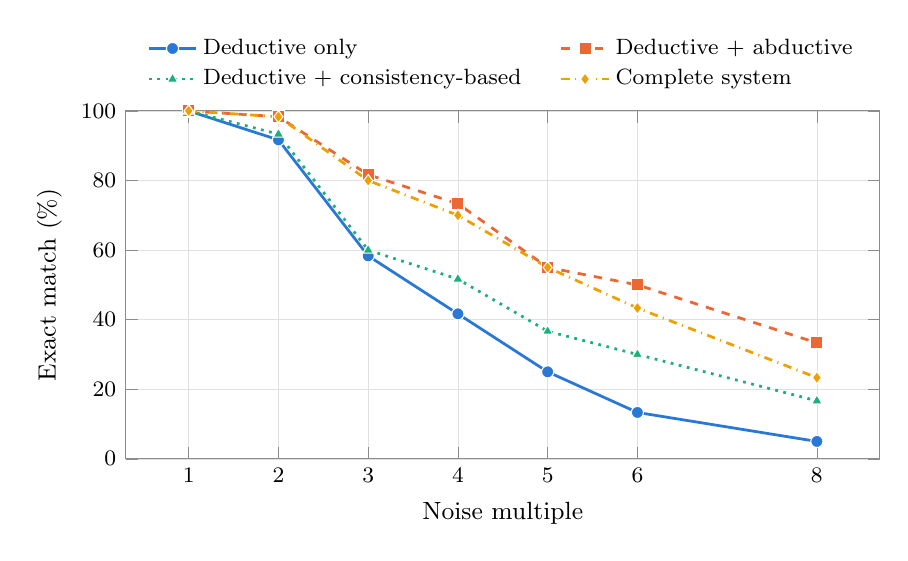
\begin{tikzpicture}
\definecolor{modedeductive}{HTML}{2a78d6}
\definecolor{modededabd}{HTML}{eb6834}
\definecolor{modededcbd}{HTML}{1baf7a}
\definecolor{modefull}{HTML}{eda100}
\begin{axis}[
  width=0.92\linewidth, height=6cm,
  xlabel={Noise multiple}, ylabel={Exact match (\%)},
  ymin=0, ymax=100,
  xtick={1,2,3,4,5,6,8},
  grid=major, major grid style={line width=0.2pt, draw=black!12},
  axis line style={draw=black!45}, tick style={draw=black!45},
  label style={font=\small}, tick label style={font=\footnotesize},
  legend style={font=\footnotesize, draw=none, fill=none, at={(0.5,1.03)}, anchor=south, legend columns=2,
    /tikz/every even column/.append style={column sep=1.2em}},
  legend cell align=left,
]
\addplot[color=modedeductive, solid, line width=1pt, mark=*, mark size=2.2pt, mark options={solid, draw=white, line width=0.4pt}] coordinates {(1,100.00) (2,91.67) (3,58.33) (4,41.67) (5,25.00) (6,13.33) (8,5.00)};
\addlegendentry{Deductive only}
\addplot[color=modededabd, dashed, line width=1pt, mark=square*, mark size=2.2pt, mark options={solid, draw=white, line width=0.4pt}] coordinates {(1,100.00) (2,98.33) (3,81.67) (4,73.33) (5,55.00) (6,50.00) (8,33.33)};
\addlegendentry{Deductive + abductive}
\addplot[color=modededcbd, dotted, line width=1pt, mark=triangle*, mark size=2.2pt, mark options={solid, draw=white, line width=0.4pt}] coordinates {(1,100.00) (2,93.33) (3,60.00) (4,51.67) (5,36.67) (6,30.00) (8,16.67)};
\addlegendentry{Deductive + consistency-based}
\addplot[color=modefull, dashdotted, line width=1pt, mark=diamond*, mark size=2.2pt, mark options={solid, draw=white, line width=0.4pt}] coordinates {(1,100.00) (2,98.33) (3,80.00) (4,70.00) (5,55.00) (6,43.33) (8,23.33)};
\addlegendentry{Complete system}
\end{axis}
\end{tikzpicture}

  \caption{Exact-match accuracy against sensor noise, by reasoning mode. Each point is 60 synthetic cases.}
  \label{fig:sens-noise}
\end{figure}

% Generated by tests/sensitivity.py. Do not edit by hand.
\begin{table}[htbp]
  \centering
  \footnotesize
  \setlength{\tabcolsep}{4pt}
  \caption{Sensitivity to sensor noise: exact match by reasoning mode, with coverage, macro F1 and mean time in milliseconds of the complete system. Each level has 60 synthetic cases. Ded.: deductive only; +Abd.: deductive and abductive; +Cons.: deductive and consistency-based; Cov.: coverage.}
  \label{tab:sens-noise}
  \begin{tabular}{lrrrrrrr}
  \toprule
  Noise multiple & Ded. & +Abd. & +Cons. & Complete & Cov. & Macro F1 & ms \\
  \midrule
  1 & 100.0\% & 100.0\% & 100.0\% & 100.0\% & 100.0\% & 1.000 & 1.36 \\
  2 & 91.7\% & 98.3\% & 93.3\% & 98.3\% & 100.0\% & 0.985 & 1.22 \\
  3 & 58.3\% & 81.7\% & 60.0\% & 80.0\% & 96.7\% & 0.894 & 1.21 \\
  4 & 41.7\% & 73.3\% & 51.7\% & 70.0\% & 95.0\% & 0.867 & 1.24 \\
  5 & 25.0\% & 55.0\% & 36.7\% & 55.0\% & 90.0\% & 0.787 & 1.42 \\
  6 & 13.3\% & 50.0\% & 30.0\% & 43.3\% & 90.0\% & 0.776 & 2.84 \\
  8 & 5.0\% & 33.3\% & 16.7\% & 23.3\% & 81.7\% & 0.693 & 5.91 \\
  \bottomrule
  \end{tabular}
\end{table}


Noise degrades deduction fastest (Figure~\ref{fig:sens-noise} and Table~\ref{tab:sens-noise}). At four times the nominal noise, deduction keeps 42\% exact match while the abductive configuration keeps 73\%. Noise is a precision problem, not a recall problem. The deductive rules still find the true fault in most noisy cases, but crisp thresholds turn noise into additional false findings. Graded evidence, scaled to the noise estimated from the case itself, and parsimony keep those findings out of the abductive explanations.

\subsection{Missing observations}

\begin{figure}[htbp]
  \centering
  % Generated by tests/sensitivity.py. Do not edit by hand.
% Needs \usepackage{pgfplots} and \pgfplotsset{compat=1.18} in the preamble.
% Colours: validated categorical palette, slots 1 to 4. Marker and dash repeat the identity.
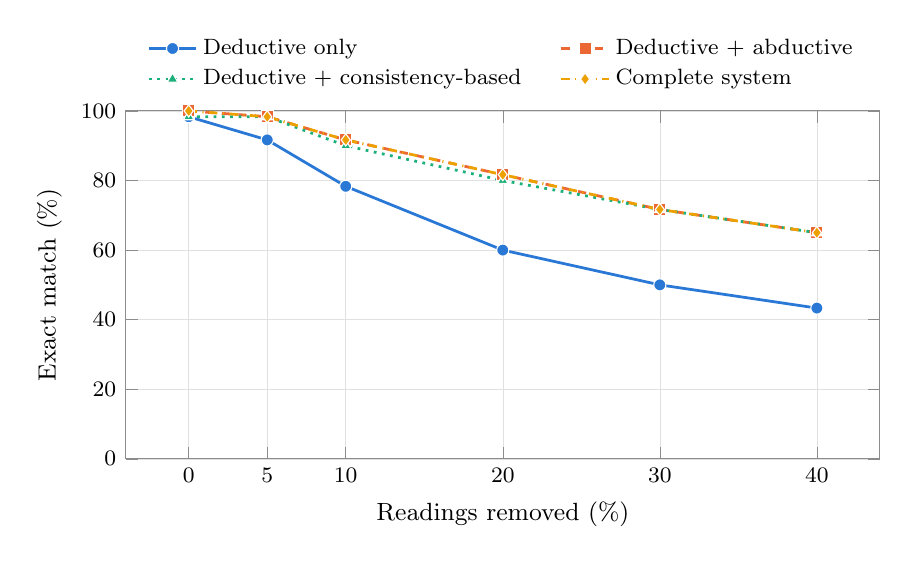
\begin{tikzpicture}
\definecolor{modedeductive}{HTML}{2a78d6}
\definecolor{modededabd}{HTML}{eb6834}
\definecolor{modededcbd}{HTML}{1baf7a}
\definecolor{modefull}{HTML}{eda100}
\begin{axis}[
  width=0.92\linewidth, height=6cm,
  xlabel={Readings removed (\%)}, ylabel={Exact match (\%)},
  ymin=0, ymax=100,
  xtick={0,5,10,20,30,40},
  grid=major, major grid style={line width=0.2pt, draw=black!12},
  axis line style={draw=black!45}, tick style={draw=black!45},
  label style={font=\small}, tick label style={font=\footnotesize},
  legend style={font=\footnotesize, draw=none, fill=none, at={(0.5,1.03)}, anchor=south, legend columns=2,
    /tikz/every even column/.append style={column sep=1.2em}},
  legend cell align=left,
]
\addplot[color=modedeductive, solid, line width=1pt, mark=*, mark size=2.2pt, mark options={solid, draw=white, line width=0.4pt}] coordinates {(0,98.33) (5,91.67) (10,78.33) (20,60.00) (30,50.00) (40,43.33)};
\addlegendentry{Deductive only}
\addplot[color=modededabd, dashed, line width=1pt, mark=square*, mark size=2.2pt, mark options={solid, draw=white, line width=0.4pt}] coordinates {(0,100.00) (5,98.33) (10,91.67) (20,81.67) (30,71.67) (40,65.00)};
\addlegendentry{Deductive + abductive}
\addplot[color=modededcbd, dotted, line width=1pt, mark=triangle*, mark size=2.2pt, mark options={solid, draw=white, line width=0.4pt}] coordinates {(0,98.33) (5,98.33) (10,90.00) (20,80.00) (30,71.67) (40,65.00)};
\addlegendentry{Deductive + consistency-based}
\addplot[color=modefull, dashdotted, line width=1pt, mark=diamond*, mark size=2.2pt, mark options={solid, draw=white, line width=0.4pt}] coordinates {(0,100.00) (5,98.33) (10,91.67) (20,81.67) (30,71.67) (40,65.00)};
\addlegendentry{Complete system}
\end{axis}
\end{tikzpicture}

  \caption{Exact-match accuracy against the share of readings removed, by reasoning mode. The three model-based configurations give almost identical results, so their lines overlap.}
  \label{fig:sens-missing}
\end{figure}

% Generated by tests/sensitivity.py. Do not edit by hand.
\begin{table}[htbp]
  \centering
  \footnotesize
  \setlength{\tabcolsep}{4pt}
  \caption{Sensitivity to missing observations: exact match by reasoning mode, with coverage, macro F1 and mean time in milliseconds of the complete system. Each level has 60 synthetic cases. Ded.: deductive only; +Abd.: deductive and abductive; +Cons.: deductive and consistency-based; Cov.: coverage.}
  \label{tab:sens-missing}
  \begin{tabular}{lrrrrrrr}
  \toprule
  Readings removed & Ded. & +Abd. & +Cons. & Complete & Cov. & Macro F1 & ms \\
  \midrule
  0\% & 98.3\% & 100.0\% & 98.3\% & 100.0\% & 100.0\% & 1.000 & 1.11 \\
  5\% & 91.7\% & 98.3\% & 98.3\% & 98.3\% & 98.3\% & 0.982 & 1.09 \\
  10\% & 78.3\% & 91.7\% & 90.0\% & 91.7\% & 91.7\% & 0.914 & 1.11 \\
  20\% & 60.0\% & 81.7\% & 80.0\% & 81.7\% & 81.7\% & 0.818 & 0.94 \\
  30\% & 50.0\% & 71.7\% & 71.7\% & 71.7\% & 71.7\% & 0.739 & 1.17 \\
  40\% & 43.3\% & 65.0\% & 65.0\% & 65.0\% & 65.0\% & 0.681 & 0.82 \\
  \bottomrule
  \end{tabular}
\end{table}


The lead of the three model-based configurations over deduction widens with the share of missing readings, from about 7 percentage points at 5\% missing to about 22 points at 20\% and beyond (Figure~\ref{fig:sens-missing}). A missing reading makes its symptom unknown rather than absent, so no hypothesis is rejected for lack of data, and a hypothesis can be accepted on its remaining evidence. A deductive rule fails as soon as one reading in its body is missing.

\subsection{Multiple simultaneous faults}

\begin{figure}[htbp]
  \centering
  % Generated by tests/sensitivity.py. Do not edit by hand.
% Needs \usepackage{pgfplots} and \pgfplotsset{compat=1.18} in the preamble.
% Colours: validated categorical palette, slots 1 to 4. Marker and dash repeat the identity.
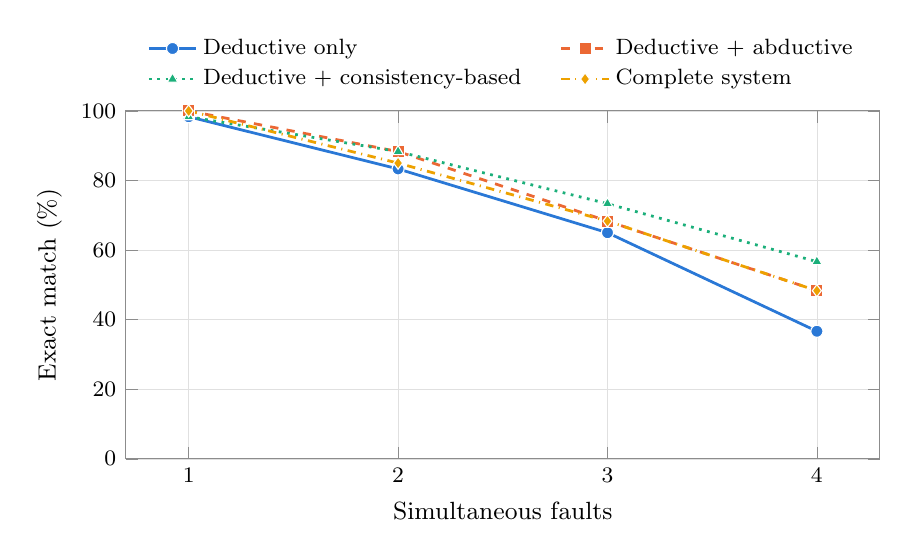
\begin{tikzpicture}
\definecolor{modedeductive}{HTML}{2a78d6}
\definecolor{modededabd}{HTML}{eb6834}
\definecolor{modededcbd}{HTML}{1baf7a}
\definecolor{modefull}{HTML}{eda100}
\begin{axis}[
  width=0.92\linewidth, height=6cm,
  xlabel={Simultaneous faults}, ylabel={Exact match (\%)},
  ymin=0, ymax=100,
  xtick={1,2,3,4},
  grid=major, major grid style={line width=0.2pt, draw=black!12},
  axis line style={draw=black!45}, tick style={draw=black!45},
  label style={font=\small}, tick label style={font=\footnotesize},
  legend style={font=\footnotesize, draw=none, fill=none, at={(0.5,1.03)}, anchor=south, legend columns=2,
    /tikz/every even column/.append style={column sep=1.2em}},
  legend cell align=left,
]
\addplot[color=modedeductive, solid, line width=1pt, mark=*, mark size=2.2pt, mark options={solid, draw=white, line width=0.4pt}] coordinates {(1,98.33) (2,83.33) (3,65.00) (4,36.67)};
\addlegendentry{Deductive only}
\addplot[color=modededabd, dashed, line width=1pt, mark=square*, mark size=2.2pt, mark options={solid, draw=white, line width=0.4pt}] coordinates {(1,100.00) (2,88.33) (3,68.33) (4,48.33)};
\addlegendentry{Deductive + abductive}
\addplot[color=modededcbd, dotted, line width=1pt, mark=triangle*, mark size=2.2pt, mark options={solid, draw=white, line width=0.4pt}] coordinates {(1,98.33) (2,88.33) (3,73.33) (4,56.67)};
\addlegendentry{Deductive + consistency-based}
\addplot[color=modefull, dashdotted, line width=1pt, mark=diamond*, mark size=2.2pt, mark options={solid, draw=white, line width=0.4pt}] coordinates {(1,100.00) (2,85.00) (3,68.33) (4,48.33)};
\addlegendentry{Complete system}
\end{axis}
\end{tikzpicture}

  \caption{Exact-match accuracy against the number of simultaneous faults, by reasoning mode.}
  \label{fig:sens-multi}
\end{figure}

% Generated by tests/sensitivity.py. Do not edit by hand.
\begin{table}[htbp]
  \centering
  \footnotesize
  \setlength{\tabcolsep}{4pt}
  \caption{Sensitivity to the number of simultaneous faults: exact match by reasoning mode, with coverage, macro F1 and mean time in milliseconds of the complete system. Each level has 60 synthetic cases. Ded.: deductive only; +Abd.: deductive and abductive; +Cons.: deductive and consistency-based; Cov.: coverage.}
  \label{tab:sens-multi}
  \begin{tabular}{lrrrrrrr}
  \toprule
  Simultaneous faults & Ded. & +Abd. & +Cons. & Complete & Cov. & Macro F1 & ms \\
  \midrule
  1 & 98.3\% & 100.0\% & 98.3\% & 100.0\% & 100.0\% & 1.000 & 1.35 \\
  2 & 83.3\% & 88.3\% & 88.3\% & 85.0\% & 93.3\% & 0.983 & 1.43 \\
  3 & 65.0\% & 68.3\% & 73.3\% & 68.3\% & 76.7\% & 0.951 & 1.40 \\
  4 & 36.7\% & 48.3\% & 56.7\% & 48.3\% & 48.3\% & 0.846 & 1.73 \\
  \bottomrule
  \end{tabular}
\end{table}


Exact-match accuracy falls as faults are combined (Figure~\ref{fig:sens-multi}). Precision stays close to 1, so the system rarely reports a fault that is not present, while recall falls as interacting faults share symptoms. Two cooling faults together, such as a fan failure and a chilled-water loss, overlap in what they show, and parsimony then prefers one fault to two. The consistency-based configuration handles four faults best, because a fault model forces it to keep a second fault whose own relation was violated. Reasoning remains fast at every fault count (Figure~\ref{fig:sens-multi-time}). The timing curves are wall-clock measurements and include some noise from other processes on the test machine, such as the dip at two faults. They should therefore be read only as an order of magnitude: a few milliseconds per case at every fault count, far below the sampling interval of data centre monitoring. Differences of a fraction of a millisecond between configurations or fault counts are not meaningful.

\begin{figure}[htbp]
  \centering
  % Generated by tests/sensitivity.py. Do not edit by hand.
% Needs \usepackage{pgfplots} and \pgfplotsset{compat=1.18} in the preamble.
% Colours: validated categorical palette, slots 1 to 4. Marker and dash repeat the identity.
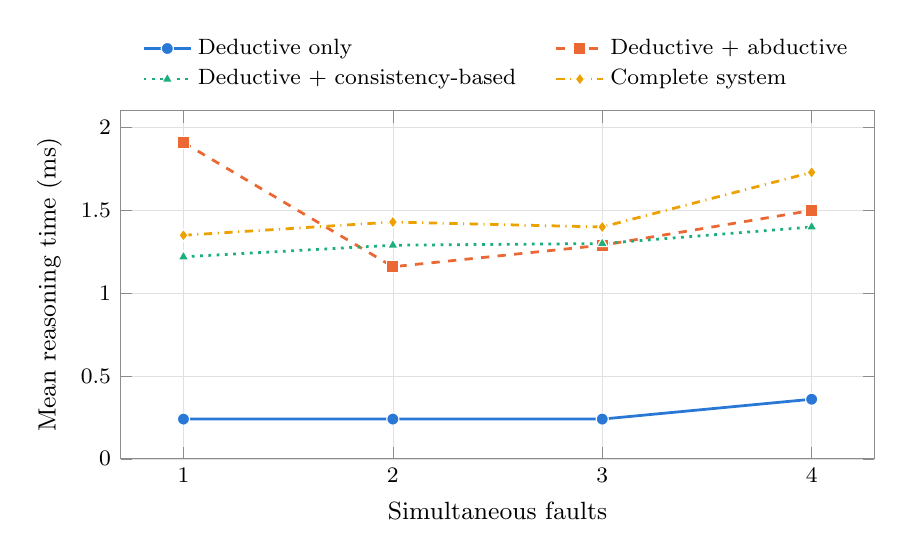
\begin{tikzpicture}
\definecolor{modedeductive}{HTML}{2a78d6}
\definecolor{modededabd}{HTML}{eb6834}
\definecolor{modededcbd}{HTML}{1baf7a}
\definecolor{modefull}{HTML}{eda100}
\begin{axis}[
  width=0.92\linewidth, height=6cm,
  xlabel={Simultaneous faults}, ylabel={Mean reasoning time (ms)},
  ymin=0,
  xtick={1,2,3,4},
  grid=major, major grid style={line width=0.2pt, draw=black!12},
  axis line style={draw=black!45}, tick style={draw=black!45},
  label style={font=\small}, tick label style={font=\footnotesize},
  legend style={font=\footnotesize, draw=none, fill=none, at={(0.5,1.03)}, anchor=south, legend columns=2,
    /tikz/every even column/.append style={column sep=1.2em}},
  legend cell align=left,
]
\addplot[color=modedeductive, solid, line width=1pt, mark=*, mark size=2.2pt, mark options={solid, draw=white, line width=0.4pt}] coordinates {(1,0.24) (2,0.24) (3,0.24) (4,0.36)};
\addlegendentry{Deductive only}
\addplot[color=modededabd, dashed, line width=1pt, mark=square*, mark size=2.2pt, mark options={solid, draw=white, line width=0.4pt}] coordinates {(1,1.91) (2,1.16) (3,1.29) (4,1.50)};
\addlegendentry{Deductive + abductive}
\addplot[color=modededcbd, dotted, line width=1pt, mark=triangle*, mark size=2.2pt, mark options={solid, draw=white, line width=0.4pt}] coordinates {(1,1.22) (2,1.29) (3,1.30) (4,1.40)};
\addlegendentry{Deductive + consistency-based}
\addplot[color=modefull, dashdotted, line width=1pt, mark=diamond*, mark size=2.2pt, mark options={solid, draw=white, line width=0.4pt}] coordinates {(1,1.35) (2,1.43) (3,1.40) (4,1.73)};
\addlegendentry{Complete system}
\end{axis}
\end{tikzpicture}

  \caption{Mean reasoning time per case against the number of simultaneous faults. Times are wall-clock and include measurement noise.}
  \label{fig:sens-multi-time}
\end{figure}

\subsection{Contradictory evidence: sensor bias}

\begin{figure}[htbp]
  \centering
  % Generated by tests/sensitivity.py. Do not edit by hand.
% Needs \usepackage{pgfplots} and \pgfplotsset{compat=1.18} in the preamble.
% Colours: validated categorical palette, slots 1 to 4. Marker and dash repeat the identity.
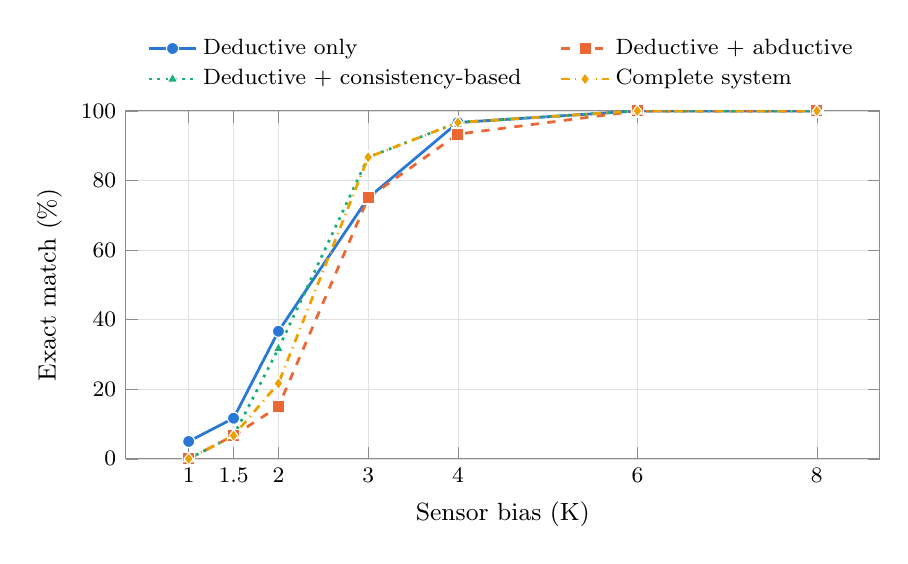
\begin{tikzpicture}
\definecolor{modedeductive}{HTML}{2a78d6}
\definecolor{modededabd}{HTML}{eb6834}
\definecolor{modededcbd}{HTML}{1baf7a}
\definecolor{modefull}{HTML}{eda100}
\begin{axis}[
  width=0.92\linewidth, height=6cm,
  xlabel={Sensor bias (K)}, ylabel={Exact match (\%)},
  ymin=0, ymax=100,
  xtick={1,1.5,2,3,4,6,8},
  grid=major, major grid style={line width=0.2pt, draw=black!12},
  axis line style={draw=black!45}, tick style={draw=black!45},
  label style={font=\small}, tick label style={font=\footnotesize},
  legend style={font=\footnotesize, draw=none, fill=none, at={(0.5,1.03)}, anchor=south, legend columns=2,
    /tikz/every even column/.append style={column sep=1.2em}},
  legend cell align=left,
]
\addplot[color=modedeductive, solid, line width=1pt, mark=*, mark size=2.2pt, mark options={solid, draw=white, line width=0.4pt}] coordinates {(1,5.00) (1.5,11.67) (2,36.67) (3,75.00) (4,96.67) (6,100.00) (8,100.00)};
\addlegendentry{Deductive only}
\addplot[color=modededabd, dashed, line width=1pt, mark=square*, mark size=2.2pt, mark options={solid, draw=white, line width=0.4pt}] coordinates {(1,0.00) (1.5,6.67) (2,15.00) (3,75.00) (4,93.33) (6,100.00) (8,100.00)};
\addlegendentry{Deductive + abductive}
\addplot[color=modededcbd, dotted, line width=1pt, mark=triangle*, mark size=2.2pt, mark options={solid, draw=white, line width=0.4pt}] coordinates {(1,0.00) (1.5,6.67) (2,31.67) (3,86.67) (4,96.67) (6,100.00) (8,100.00)};
\addlegendentry{Deductive + consistency-based}
\addplot[color=modefull, dashdotted, line width=1pt, mark=diamond*, mark size=2.2pt, mark options={solid, draw=white, line width=0.4pt}] coordinates {(1,0.00) (1.5,6.67) (2,21.67) (3,86.67) (4,96.67) (6,100.00) (8,100.00)};
\addlegendentry{Complete system}
\end{axis}
\end{tikzpicture}

  \caption{Exact-match accuracy against the size of an injected temperature-sensor bias.}
  \label{fig:sens-bias}
\end{figure}

% Generated by tests/sensitivity.py. Do not edit by hand.
\begin{table}[htbp]
  \centering
  \footnotesize
  \setlength{\tabcolsep}{4pt}
  \caption{Sensitivity to the size of a sensor bias, a source of contradictory evidence: exact match by reasoning mode, with coverage, macro F1 and mean time in milliseconds of the complete system. Each level has 60 synthetic cases. Ded.: deductive only; +Abd.: deductive and abductive; +Cons.: deductive and consistency-based; Cov.: coverage.}
  \label{tab:sens-bias}
  \begin{tabular}{lrrrrrrr}
  \toprule
  Sensor bias & Ded. & +Abd. & +Cons. & Complete & Cov. & Macro F1 & ms \\
  \midrule
  1\,K & 5.0\% & 0.0\% & 0.0\% & 0.0\% & 0.0\% & 0.000 & 0.96 \\
  1.5\,K & 11.7\% & 6.7\% & 6.7\% & 6.7\% & 6.7\% & 0.121 & 1.06 \\
  2\,K & 36.7\% & 15.0\% & 31.7\% & 21.7\% & 21.7\% & 0.317 & 1.05 \\
  3\,K & 75.0\% & 75.0\% & 86.7\% & 86.7\% & 86.7\% & 0.929 & 1.11 \\
  4\,K & 96.7\% & 93.3\% & 96.7\% & 96.7\% & 96.7\% & 0.983 & 1.13 \\
  6\,K & 100.0\% & 100.0\% & 100.0\% & 100.0\% & 100.0\% & 1.000 & 1.18 \\
  8\,K & 100.0\% & 100.0\% & 100.0\% & 100.0\% & 100.0\% & 1.000 & 1.63 \\
  \bottomrule
  \end{tabular}
\end{table}


A biased sensor contradicts its neighbours and the energy balances. Biases below the 2\,K neighbour-deviation threshold are rarely detected, which is the expected limit of the design, and biases of 4\,K or more are detected almost always (Figure~\ref{fig:sens-bias}). At 3\,K the consistency-based configurations do best, because a single sensor fault is then the only minimal diagnosis that removes every conflict. At 2\,K the graded modes are deliberately more cautious than deduction, because they require one noise standard deviation of margin past the threshold.

\subsection{Threshold changes}

Each threshold was perturbed on its own on the held-out split (Table~\ref{tab:sens-thresholds}). Eleven of the 23 thresholds change nothing at any level, because backup rules or other symptoms cover them, or because no case lies near them. At $\pm$1\,K or $\pm$10\%, all but three change the complete system's accuracy by less than 3 percentage points.

% Generated by tests/sensitivity.py from docs/10b_threshold_sensitivity.md. Do not edit by hand.
\begin{footnotesize}
\setlength{\tabcolsep}{4pt}
\begin{longtable}{L{4.4cm}L{1.6cm}rrrrr}
  \caption{Threshold sensitivity on the held-out split: change in exact-match accuracy of the complete system, in percentage points, when one threshold is perturbed. Temperature thresholds move by $-2$, $-1$, $+1$ and $+2$\,K; other thresholds are scaled by 0.8, 0.9, 1.1 and 1.2. The last column is the worst change for deduction alone. A dot means no change.}\label{tab:sens-thresholds}\\
  \toprule
  Threshold & Base & $-2$ / 0.8 & $-1$ / 0.9 & $+1$ / 1.1 & $+2$ / 1.2 & Ded. worst \\
  \midrule
  \endfirsthead
  \toprule
  Threshold & Base & $-2$ / 0.8 & $-1$ / 0.9 & $+1$ / 1.1 & $+2$ / 1.2 & Ded. worst \\
  \midrule
  \endhead
  \texttt{t\_\allowbreak{}inlet\_\allowbreak{}rec\_\allowbreak{}max} & 27.0 \textdegree C & $\cdot$ & $\cdot$ & $\cdot$ & $\cdot$ & $\cdot$ \\
  \texttt{t\_\allowbreak{}inlet\_\allowbreak{}rec\_\allowbreak{}min} & 18.0 \textdegree C & $\cdot$ & $\cdot$ & $\cdot$ & $\cdot$ & $\cdot$ \\
  \texttt{t\_\allowbreak{}supply\_\allowbreak{}band} & 2.0 K & $\cdot$ & $\cdot$ & $\cdot$ & $\cdot$ & -7.5 \\
  \texttt{row\_\allowbreak{}hot\_\allowbreak{}fraction} & 0.5 & $\cdot$ & $\cdot$ & $\cdot$ & $\cdot$ & $\cdot$ \\
  \texttt{valve\_\allowbreak{}open\_\allowbreak{}min} & 50.0 \% & $\cdot$ & $\cdot$ & $\cdot$ & $\cdot$ & $\cdot$ \\
  \texttt{chw\_\allowbreak{}flow\_\allowbreak{}ratio\_\allowbreak{}min} & 0.3 & -0.8 & -0.8 & $\cdot$ & $\cdot$ & $\cdot$ \\
  \texttt{strat\_\allowbreak{}max} & 3.0 K & -77.3 & -2.7 & $\cdot$ & -0.8 & -90.2 \\
  \texttt{fan\_\allowbreak{}ratio\_\allowbreak{}min} & 0.5 & $\cdot$ & $\cdot$ & $\cdot$ & $\cdot$ & $\cdot$ \\
  \texttt{strat\_\allowbreak{}out\_\allowbreak{}max} & 3.5 K & -50.2 & -1.2 & -4.3 & -8.2 & -76.5 \\
  \texttt{filter\_\allowbreak{}loading\_\allowbreak{}max} & 1.7 & 0.8 & $\cdot$ & -0.8 & -2.0 & -1.2 \\
  \texttt{server\_\allowbreak{}fan\_\allowbreak{}min} & 1000.0 rpm & $\cdot$ & $\cdot$ & $\cdot$ & $\cdot$ & $\cdot$ \\
  \texttt{cpu\_\allowbreak{}hot\_\allowbreak{}min} & 85.0 \textdegree C & $\cdot$ & $\cdot$ & $\cdot$ & $\cdot$ & $\cdot$ \\
  \texttt{branch\_\allowbreak{}loading\_\allowbreak{}max} & 0.8 & 0.8 & 0.8 & -3.9 & -9.0 & -9.0 \\
  \texttt{cell\_\allowbreak{}r\_\allowbreak{}ratio\_\allowbreak{}max} & 1.3 & -30.2 & 0.8 & -0.4 & -0.8 & -43.9 \\
  \texttt{ups\_\allowbreak{}eff\_\allowbreak{}bypass\_\allowbreak{}min} & 0.98 & -84.3 & -83.9 & $\cdot$ & $\cdot$ & -1.2 \\
  \texttt{neighbour\_\allowbreak{}dev\_\allowbreak{}max} & 2.0 K & -85.1 & -0.4 & $\cdot$ & $\cdot$ & -87.8 \\
  \texttt{balance\_\allowbreak{}resid\_\allowbreak{}max} & 0.2 & $\cdot$ & $\cdot$ & $\cdot$ & $\cdot$ & $\cdot$ \\
  \texttt{sample\_\allowbreak{}age\_\allowbreak{}max} & 60.0 s & $\cdot$ & $\cdot$ & $\cdot$ & $\cdot$ & $\cdot$ \\
  \texttt{t\_\allowbreak{}supply\_\allowbreak{}hot\_\allowbreak{}limit} & 22.0 \textdegree C & -12.5 & $\cdot$ & $\cdot$ & $\cdot$ & $\cdot$ \\
  \texttt{fan\_\allowbreak{}ratio\_\allowbreak{}reduced} & 0.85 & $\cdot$ & $\cdot$ & $\cdot$ & -45.5 & -7.1 \\
  \texttt{t\_\allowbreak{}supply\_\allowbreak{}cold\_\allowbreak{}limit} & 18.0 \textdegree C & $\cdot$ & $\cdot$ & $\cdot$ & -11.4 & $\cdot$ \\
  \texttt{power\_\allowbreak{}resid\_\allowbreak{}max} & 0.1 & -0.4 & $\cdot$ & 0.4 & 0.4 & $\cdot$ \\
  \texttt{sensor\_\allowbreak{}noise\_\allowbreak{}floor} & 0.15 K & $\cdot$ & $\cdot$ & $\cdot$ & $\cdot$ & $\cdot$ \\
  \bottomrule
\end{longtable}
\end{footnotesize}


The large drops share one cause: each occurs when the perturbed threshold moves inside the scatter of normal operation. Moving the inlet stratification limit to 1\,K, inside the 1 to 2.2\,K of sealed racks, costs 77 points. Scaling the reduced-fan-power limit to 1.02, inside the $\pm$5\% scatter of a healthy fan, costs 46 points. This is evidence that each threshold sits in a margin between the normal envelope and the fault envelope, and the table measures how wide each margin is.

One result is a warning about consistency checking. Scaling the UPS-efficiency threshold to 0.88 puts every healthy double-conversion UPS, which runs near 0.955, above it. Deduction loses only 1.2 points, because its UPS rule relies on the mode flag. The complete system loses 84 points, because the mis-set relation produces a conflict in every case and the consistency module then rejects every correct explanation. A redundancy relation acts as a hard constraint, so a wrong relation threshold corrupts every diagnosis. Relation thresholds should therefore be derived from sensor uncertainty (Equation~\eqref{eq:uncertainty}) and validated on normal data before deployment.

\subsection{Reasoning parameters}
\label{sec:param-sensitivity}

The threshold study does not cover the five reasoning parameters set by judgement (Table~\ref{tab:design-params}). Each was changed on its own, and the three model-based configurations were run on both splits and on four stress sets from this section: four times the nominal noise, 20\% of readings missing, four simultaneous faults, and a 2\,K sensor bias, which lies in the transition between missed and detected biases. Table~\ref{tab:param-sensitivity} gives the results. Deduction uses none of these parameters and is the reference. The study is generated by \texttt{tests/param\_sensitivity.py}.

% Generated by tests/param_sensitivity.py. Do not edit by hand.
\begin{table}[htbp]
  \centering
  \scriptsize
  \setlength{\tabcolsep}{3pt}
  \caption{Sensitivity to the reasoning parameters set by judgement. Each parameter is changed alone. The first two rows give exactly matched cases at the defaults; the other rows give the change in exactly matched cases, for deductive + abductive / deductive + consistency-based / complete system. For the perturbed weights, the range over five random draws is given in brackets. Defaults: bonus 0.1, cut-off $k = 1$, search bound 4, weights from \texttt{kb/causal.pl}, noise of unredundant features tied to $\sigma_T$. Raw counts are in \texttt{docs/15\_parameter\_sensitivity.md}.}
  \label{tab:param-sensitivity}
  \begin{tabular}{L{2.3cm}lcccccc}
  \toprule
  Parameter & Value & Calibration & Held-out & Noise $\times$4 & 20\% missing & Four faults & 2 K bias \\
  \midrule
  Deduction only & & 230 & 232 & 25 & 36 & 22 & 22 \\
  Model-based & default & 238/234/238 & 241/238/239 & 44/31/42 & 49/48/49 & 29/34/29 & 9/19/13 \\
  \midrule
  Deductive bonus & 0 & 0/0/0 & 0/0/0 & 0/0/0 & 0/0/0 & 0/0/0 & 0/0/0 \\
   & 0.05 & 0/0/0 & 0/0/0 & 0/0/0 & 0/0/0 & 0/0/0 & 0/0/0 \\
   & 0.2 & 0/0/0 & +1/0/+1 & +1/0/+1 & 0/0/0 & 0/0/0 & 0/0/0 \\
   & 0.5 & 0/0/0 & +2/0/+2 & +1/0/+1 & 0/0/0 & 0/0/0 & +6/0/+6 \\
  \addlinespace
  Cut-off $k$ & 0.5 & $-$3/$-$1/$-$2 & $-$3/$-$4/$-$4 & $-$7/$-$7/$-$9 & 0/0/0 & 0/0/0 & +6/+4/+9 \\
   & 1.5 & 0/+1/0 & +1/$-$1/+1 & +2/+4/+4 & 0/0/0 & 0/0/0 & $-$2/$-$2/$-$3 \\
   & 2.0 & +1/+1/+1 & +1/+2/+2 & +3/+6/+5 & 0/0/0 & 0/0/0 & $-$2/$-$4/$-$5 \\
  \addlinespace
  Search bound & 2 & 0/0/0 & 0/+1/0 & +1/+1/0 & 0/0/0 & $-$29/$-$12/$-$29 & 0/0/0 \\
   & 3 & 0/0/0 & 0/0/0 & +1/0/0 & 0/0/0 & $-$29/$-$12/$-$29 & 0/0/0 \\
   & 5 & 0/0/0 & 0/0/0 & 0/0/0 & 0/0/0 & 0/$-$4/0 & 0/0/0 \\
  \addlinespace
  Causal weights & all 1 & 0/0/0 & 0/0/0 & 0/0/0 & $-$1/0/$-$1 & 0/0/0 & 0/0/0 \\
   & $\times$U[.5,1.5] & $-$1/0/$-$1 & 0/0/0 & 0/0/0 & [0,+1]/0/[0,+1] & 0/0/0 & 0/0/0 \\
  \addlinespace
  Noise scaling & fixed & +1/+1/+1 & 0/0/0 & $-$1/$-$3/$-$4 & 0/0/0 & 0/0/0 & 0/0/0 \\
  \bottomrule
  \end{tabular}
\end{table}


\begin{itemize}
  \item \textbf{Causal weights hardly matter.} Setting every weight to 1, or multiplying each by a random factor between 0.5 and 1.5 in five independent draws, changes at most one case on any set. Parsimony, not the weights, decides most explanations, and the weights only rank explanations of the same size.
  \item \textbf{The deductive bonus hardly matters up to 0.2.} At 0.5 it gains two held-out cases and six 2\,K-bias cases, because abduction then defers to the rules, which detect small biases better (Section~\ref{sec:sensitivity}). It leaves the calibration split unchanged.
  \item \textbf{The evidence cut-off is a real trade-off.} A looser cut-off, $k = 0.5$, catches four to nine more 2\,K biases but loses seven to nine cases under heavy noise. A stricter one, $k = 2$, gains three to six noisy cases and loses two to five small biases. The default $k = 1$ lies between them: on the held-out split it is at most two cases behind the stricter cut-off and three or four ahead of the looser one.
  \item \textbf{The search bound must cover the largest fault combination.} A bound of 2 or 3 loses every four-fault case of the abductive configurations, and 12 of the consistency-based one. A bound of 5 changes nothing, except that consistency-based search then accepts larger, wrong diagnoses in four of the four-fault cases.
  \item \textbf{Tying the noise of unredundant features to the temperature sensors helps under noise.} With fixed nominal noise instead, the model-based configurations lose one to four cases at four times the noise, and gain one calibration case.
\end{itemize}

The defaults were set before this study and were not changed after it. The held-out split must not be used to tune them, and on the calibration split no variant except the search bound and the loosest cut-off moves any configuration by more than one case, so the calibration data give no reason to change them either. The results support the claim that the conclusions of this chapter do not depend on the exact values chosen by judgement, except for the evidence cut-off, which sets the balance between robustness to noise and sensitivity to small faults.

\subsection{Summary}

Table~\ref{tab:sens-summary} summarises the findings of the sensitivity and ablation analysis.

\begin{table}[htbp]
  \centering
  \small
  \caption{Summary of the sensitivity analysis.}
  \label{tab:sens-summary}
  \begin{tabular}{L{4.2cm}L{9.8cm}}
    \toprule
    Question & Finding \\
    \midrule
    Threshold changes & Robust within $\pm$1\,K or $\pm$10\%. Large losses only when a threshold enters normal scatter. Consistency checking is sensitive to wrong relation thresholds. \\
    Missing observations & The model-based configurations lead deduction by about 7 points at 5\% missing, widening to about 22 points at 20\% and beyond. \\
    Contradictory evidence & Sensor biases of 3\,K and more are reliably found; consistency checking is best at the detection limit. \\
    Noisy data & Abduction with noise-adaptive evidence is the most robust configuration. \\
    Multiple faults & Precision stays near 1; recall falls with the number of faults because interacting faults share symptoms. \\
    Reasoning parameters & Causal weights and the deductive bonus hardly matter. The evidence cut-off trades robustness to noise against sensitivity to small faults. The search bound must cover the largest fault combination. \\
    Reasoning time & A few milliseconds per case in every sweep. \\
    \bottomrule
  \end{tabular}
\end{table}

% ---------------------------------------------------------------------------
\section{Robustness to Model Mismatch}
\label{sec:mismatch}

Every result so far was obtained on cases generated by the same engineering model that the knowledge base encodes. This section asks how much the diagnosis depends on that model being exactly right.

\paragraph{Method.} The 255 held-out cases were regenerated with the same seed, and so with the same faults, severities and random draws, but with deliberately changed simulator physics. Table~\ref{tab:mismatch-profiles} lists the two profiles. They change the coil heat transfer, server power and airflow, CPU thermal behaviour, the share of airflow shortfall drawn from the hot aisle, natural recirculation, room temperature, fan-control margin and sensor noise. Equipment ratings that a real knowledge base would take from nameplates, such as the fan's rated power and the valve characteristic, were left unchanged. The knowledge base was not modified. Because each case keeps its faults and draws, the results are compared with the nominal split case by case.

\begin{table}[htbp]
  \centering
  \small
  \caption{Simulator physics in the two model-mismatch profiles.}
  \label{tab:mismatch-profiles}
  \begin{tabular}{L{6.8cm}rrr}
    \toprule
    Parameter & Nominal & Mild & Strong \\
    \midrule
    Coil air-side conductance (kW/K) & 15 & 12 & 10 \\
    Coil water-side conductance at design flow (kW/K) & 10 & 12 & 14 \\
    Server idle and full-load power (kW) & 0.40, 0.90 & 0.35, 0.95 & 0.30, 1.05 \\
    Server airflow at nominal fan speed (kg/s) & 0.055 & 0.050 & 0.045 \\
    CPU share of server power & 0.55 & 0.50 & 0.60 \\
    CPU thermal resistance (K/kW) & 90 & 90 & 110 \\
    Share of airflow shortfall from the hot aisle & 0.4 & 0.5 & 0.6 \\
    Natural recirculation at the top of a sealed rack & 0.10 & 0.12 & 0.15 \\
    Fan-control airflow margin & 1.10 & 1.15 & 1.25 \\
    Room air temperature (\textdegree C) & 25 & 26 & 27 \\
    Sensor noise, multiple of nominal & 1.0 & 1.25 & 1.5 \\
    \bottomrule
  \end{tabular}
\end{table}

% Generated by tests/mismatch.py. Do not edit by hand.
\begin{table}[htbp]
  \centering
  \footnotesize
  \setlength{\tabcolsep}{4pt}
  \caption{Model mismatch: exact match of each reasoning mode when the held-out cases are regenerated with changed simulator physics and diagnosed with the unchanged knowledge base. The last pair of columns re-baselines three envelope thresholds from normal operating data only. $p$: exact McNemar test against the nominal split, paired case by case. Confidence intervals are in \texttt{docs/12\_model\_mismatch.md}.}
  \label{tab:mismatch}
  \begin{tabular}{L{3.2cm}rrrrrrr}
  \toprule
  Mode & Nominal & Mild & $p$ & Strong & $p$ & Re-baselined & $p$ \\
  \midrule
  Deductive only & 91.0\% & 80.8\% & \textbf{\textless\,0.001} & 26.3\% & \textbf{\textless\,0.001} & 75.3\% & \textbf{\textless\,0.001} \\
  Deductive + abductive & 94.5\% & 91.0\% & \textbf{0.004} & 40.0\% & \textbf{\textless\,0.001} & 83.1\% & \textbf{\textless\,0.001} \\
  Deductive + consistency-based & 93.3\% & 86.3\% & \textbf{\textless\,0.001} & 33.7\% & \textbf{\textless\,0.001} & 83.5\% & \textbf{\textless\,0.001} \\
  Complete system & 93.7\% & 90.2\% & \textbf{0.004} & 39.6\% & \textbf{\textless\,0.001} & 82.4\% & \textbf{\textless\,0.001} \\
  \bottomrule
  \end{tabular}
\end{table}

% Generated by tests/mismatch.py. Do not edit by hand.
\begin{table}[htbp]
  \centering
  \small
  \caption{Model mismatch by test category: exact matches of the complete system.}
  \label{tab:mismatch-categories}
  \begin{tabular}{L{3.4cm}rrrrr}
  \toprule
  Category & Cases & Nominal & Mild & Strong & Re-baselined \\
  \midrule
  Normal & 30 & 30 & 30 & 13 & 30 \\
  Single faults & 120 & 120 & 117 & 57 & 111 \\
  Instrumentation & 30 & 30 & 29 & 6 & 29 \\
  Multiple faults & 30 & 29 & 28 & 14 & 17 \\
  Incomplete & 15 & 14 & 13 & 5 & 13 \\
  High noise & 15 & 7 & 4 & 1 & 3 \\
  Borderline & 15 & 9 & 9 & 5 & 7 \\
  \bottomrule
  \end{tabular}
\end{table}


\paragraph{Mild mismatch.} With the physics changed by about 10 to 25\%, the configurations with abduction lose about four points of exact-match accuracy, keeping 90 to 91\%, while deduction alone falls from 91.0\% to 80.8\% (Table~\ref{tab:mismatch}). Every configuration loses significantly, but graded, noise-adaptive evidence makes the model-based configurations markedly less sensitive to model error than crisp rules.

\paragraph{Strong mismatch.} With changes of about 25 to 50\%, every configuration collapses, to between 26\% and 40\%. Even 17 of the 30 normal cases are misdiagnosed (Table~\ref{tab:mismatch-categories}). Inspection of the failures shows that the reasoning is intact and that three envelope thresholds are to blame. With less airflow per server and more natural recirculation, healthy racks stratify by 3 to 4\,K, above the 3\,K and 3.5\,K stratification thresholds. With hotter-running CPUs, healthy servers exceed the 85\,\textdegree C CPU threshold. The system then sees recirculation where there is none, or symptoms that no hypothesis explains. The thresholds encode the normal envelope of the nominal model, and the strong profile moves that envelope.

\paragraph{Re-baselining from normal operating data.} A real site has plenty of data from normal operation, even when it has no fault data. To test whether that is enough, normal-only cases were generated under the strong physics with a different seed (20261020). Each of the three envelope thresholds was shifted by how far the largest normal value moved, which keeps its original margin above normal operation. No fault labels were used. The shifts were $+2.3$\,K and $+2.2$\,K for the inlet and outlet stratification thresholds and $+26.7$\,K for the CPU threshold. Re-baselining restores the complete system to 82.4\% and the other model-based configurations to about 83\%, against 75.3\% for deduction. Normal and instrumentation cases are again almost all correct. Multiple faults, at 17 of 30, and high-noise cases recover only partly. The re-baselined CPU threshold also lies above the throttling limit, so CPU temperature no longer helps to detect a failed server fan.

\paragraph{Implication.} The diagnostic reasoning transfers across models, but fixed absolute thresholds do not. A deployment would therefore need its envelope thresholds calibrated against the site's own normal operation before use. Defining those thresholds relative to a learned baseline, rather than as fixed values, is the most direct improvement this experiment suggests (Section~\ref{sec:future}).

% ---------------------------------------------------------------------------
\section{Comparison with a Data-Driven Baseline}
\label{sec:baseline}

Fault diagnosis in data centres has mostly been data-driven (Chapter~\ref{ch:theory_and_kr}), and this project offers explainability instead. That trade-off should be shown, not asserted. Standard classifiers were therefore trained on the raw readings, with no engineering knowledge, and tested on the same cases as the expert system. The framework forbids replacing the symbolic system with machine learning, not comparing against it, so the classifiers are a baseline only and play no part in the expert system.

\paragraph{Method.} Each case becomes one vector of every reading, with a missing reading left missing. The labels are the fault labels seen in training, such as chw\_supply\_loss(crah\_1), learned as one binary output each. A case with no predicted fault is predicted normal. A random forest of 300 trees and a single decision tree were trained with the standard settings of scikit-learn \parencite{pedregosa2011}, without tuning, in two regimes: on the calibration split, the 255 cases against which the knowledge base was checked, and on 2550 further simulated cases, far more labelled fault data than a real site would have. The second regime favours the classifiers in two ways: they see labelled examples of nearly every fault at every location, and they are trained and tested on the same simulator. The script is \texttt{tests/baseline.py}.

% Generated by tests/baseline.py. Do not edit by hand.
\begin{table}[htbp]
  \centering
  \footnotesize
  \setlength{\tabcolsep}{4pt}
  \caption{Exact match of the expert system and of data-driven classifiers trained on the raw readings, on the same test cases (255 held-out, 1275 over five seeds, 255 per mismatch profile). The classifiers are a baseline for comparison only. Bold: significantly different from deductive + abductive reasoning on the same cases (exact McNemar, $p < 0.05$). Details in \texttt{docs/17\_baseline\_comparison.md}.}
  \label{tab:baseline}
  \begin{tabular}{L{3.5cm}L{3.0cm}rrrr}
  \toprule
  System & Training data & Held-out & Five seeds & Mild mismatch & Strong mismatch \\
  \midrule
  Deductive + abductive & none & 94.5 & 93.6 & 91.0 & 40.0 \\
  Complete system & none & 93.7 & 92.9 & 90.2 & 39.6 \\
  \midrule
  Random forest & calibration (255) & \textbf{53.3} & \textbf{52.1} & \textbf{34.9} & \textbf{23.9} \\
  Decision tree & calibration (255) & \textbf{53.7} & \textbf{57.9} & \textbf{38.0} & \textbf{29.0} \\
  Random forest & 2550 extra cases & \textbf{82.0} & \textbf{82.0} & \textbf{48.6} & \textbf{30.6} \\
  Decision tree & 2550 extra cases & \textbf{89.4} & \textbf{87.1} & \textbf{50.2} & 38.0 \\
  \bottomrule
  \end{tabular}
\end{table}


Table~\ref{tab:baseline} gives the results. Four findings stand out.

\begin{itemize}
  \item \textbf{With the data the knowledge base was checked against, the classifiers fail.} Trained on the 255 calibration cases, they reach 52 to 58\% exact match. A fault label names its location, so there are dozens of labels with a few examples each, and 23 held-out cases contain a label never seen in training. No instrumentation case and only 2 of the 30 multiple-fault cases are diagnosed correctly.
  \item \textbf{With ten times as much labelled data, they come closer but stay significantly behind.} Trained on 2550 cases, the decision tree reaches 89.4\% on the held-out split and 87.1\% over five seeds, against 94.5\% and 93.6\% for deductive + abductive reasoning. The random forest, at 82.0\%, does worse than the single tree with these untuned settings. The classifiers do better than the expert system on borderline and high-noise cases: the forest gets 12 and 13 of 15 right against 9 and 9. Boundaries learned from labelled data fit the simulator's noise better than thresholds set by engineering judgement, and that is the price of sourced, explainable thresholds.
  \item \textbf{Under model mismatch, the classifiers collapse first.} With the physics changed by 10 to 25\%, the classifiers trained on 2550 cases fall to about 50\%, while deductive + abductive reasoning keeps 91.0\%. The classifiers have learned the exact envelope of the nominal simulator, not the physics behind it. Under strong mismatch every system fails, and the best classifier, at 38.0\%, is not significantly different from the expert system, at 40.0\%.
  \item \textbf{The classifiers explain nothing.} They give no proof, no competing hypotheses and no maintenance plan, they need labelled examples of every fault at every location, and they cannot diagnose a fault at a location absent from their training data.
\end{itemize}

On these data, then, the knowledge-based system is more accurate than standard classifiers, needs no labelled fault data, and transfers far better to a changed model, while also explaining every diagnosis. The classifiers' advantage on borderline and noisy cases is the strongest argument for learning thresholds from data within the symbolic system, as Section~\ref{sec:future} proposes, rather than for replacing it.

